%!TEX root = ../../dissertation.tex
%%%%%%%%%%%%%%%%%%%%%%%%%%%%%%%%%%%%%%%%%%%%%%%%%%%%%%%%%%%%%%%%%%%%%%%%%%%%%%%%
\section{Cross-Layer Information Exchange}
\label{c5:sec:crosslayerhinting}

The Internet has its historic roots deep in wired networks with a slim and well-defined network stack represented by the \acrshort{ISO}/\acrshort{OSI} or \gls{TCP}/\gls{IP} model. These layers are isolated against each other. Only predefined information exchange points, or \gls{osiSAP}, at the layer borders allow for vertical communication. A typical wired \gls{TCP}/\gls{IP} Internet environment rests atop of either an Ethernet or other access technologies, e.g., \acrshort{DSL}, \acrshort{DOCSIS} or \acrshort{PON}, at the physical and link layers.

Application layer protocols often implicitly rely on the presence and characteristics of specific lower layer protocols. Though, through the layer isolation no application can precisely know or even control the current state of the lower layers. Nonetheless, they usually make assumptions on the composition and behavior of the lower layers and plan their work accordingly. 

But the access technology diversity has strongly increased through the advent of wireless technologies, and fixed access behavioral patterns, which were examined in the past, may not be applicable any more today. The protocols used for the radio transmissions behave very differently when compared to plain Ethernet and higher layers may make false assumptions. Examples for this were given in the discussion of the stack's influences in Section~\ref{c5:sec:stack-influences}.

It would be very desirable for transport and application layer mechanisms to be able to better understand these layers and cope with these effects. The term \textit{cross-layer interactions} or \textit{cross layer information exchange} subsumes these approaches. Specific information from one layer is made available to other interested neighboring or more distant layers. Using cross-layer techniques many of the previously introduced negative layer influences can be diminished or neutralized altogether.

The next sections describe related mechanisms in the literature, classifications and then proceed to describe a new cross-layer approach that facilitates cross-layer information to the benefit of mobile streaming. The cross-layer work presented here is meant as an initial proposal to be integrated into future streaming players and their playback and transmission strategies. Therefore, no complete implementation or evaluation is given.


%%%%%%%%%%%%%%%%%%%%%%%%%%%%%%%%%%%%%%%%%%%%%%%%%%%%%%%%%%%%%%%%%%%%%%%%%%%%%%%%
\subsection{Related Cross-Layer Approaches and Classifications}

The idea of exchanging information between layers is not a particularly new one. Some specific ideas have been implemented a long time ago. The authors of \cite{Raisinghani2004720} list a number of scenarios in which cross-layer information could be used and also talk about the type of information to be shared between layers. One of the oldest and most well known cross-layer approaches is probably \gls{ECN}~\cite{rfc3168}. Here, the \gls{IP} layer of intermediate hops can signal the end nodes' \gls{TCP} layer that congestion is occurring and \gls{TCP} does not need to wait for implicit congestion signals, e.g., duplicate acknowledgments or timeouts. However, \gls{ECN} is disabled in almost every implementation by default as it lead to numerous problems and triggered bugs\footnote{\url{http://lkml.iu.edu//hypermail/linux/kernel/0009.1/0329.html}}. This is a risk that many cross-layer attempts may face.

A significant amount of publications is dealing with cross-layer information in wireless and mobile protocol stacks. A number of architectures have been proposed, e.g., \cite{raisinghani2004eclair}, \cite{1580937}, \cite{wang2003multi}, \cite{1200522}, and \cite{krishna2007cross}, but no actual solution seems to have been implemented in any of these.

While cross-layer typically implies a solely \textbf{vertical} --- meaning between network layers --- exchange flow there can also be \textbf{horizontal} --- between network nodes --- components present. \gls{DLEP}~\cite{ietf2013dlepdraft,6379143} is such an example of a \textbf{diagonal} flow, providing information of a lower layer of one entity to a higher layer at another node. For example, \gls{DLEP} can forward information available only to the (external) wireless modem or other interfaces to the routing entity of a node upon which it can act. Link characteristics such as bandwidth, latency, connection status, or information regarding neighbors can be requested.

Though, horizontal information flow in cross-layer approaches is more than often an indication of \textbf{centralization} (also called \textbf{network-assisted} or \textbf{managed}) as apposed to purely vertical \textbf{distributed} approaches. Concerning this network-assisted cross-layer exchange there are a number of approaches that aim to integrate layer cooperation into the design of new mobile network infrastructures, including \cite{zarai2010seamless} and \cite{Piamrat20111066}. Generally, information is retrieved from the clients and collected at a central manager to be used in any policy decision like mobility and radio resource management.

Going back to purely distributed approaches, in \cite{hummel2010mobilitaet} the concept of mobility awareness is discussed. The goal is to predict device motion and mobility based on available information and adapt the individual network layers to react accordingly. One of the easiest mechanisms to implement the usage of cross-layer information for is the selection of the active network interface. Current mobile devices have a wide range of network interfaces available, all with specific characteristics. The management architecture proposed in  \cite{Bonnin:2009:AMM:1503496.1503498} switches the currently used interface based on pre-configured profiles. Information from multiple layers is used to support the decision-making process.

To optimize unreliable video streaming in a WiFi network, the authors of \cite{1580941} create a control loop between the video encoder and the 802.11 \gls{MAC} layer to conduct WiFi rate control fitted to the output of the encoder. This is an example of a tight cross-layer control loop for one particular application. The link layer rate control will very likely have adverse affects on other applications using this node.

The notion of cross-layer can also be applied to non-traditional network stacks. For example, the authors of \cite{4656786} present a cross-layer model for satellite communication stacks. They additionally distinguish between two general flavors of cross-layer architectures, one with \textbf{direct} and the other with \textbf{indirect} communication. Direct exchange implements new vertical interfaces in the layers and exchanges information directly between them. The indirect alternative uses an external information broker that handles all communication in parallel to the existing layers. Similar cross-layer information can be offered to peer-to-peer overlay networks, as was for example researched in the SmoothIT project\footnote{\url{http://www.smoothit.org}}, where routing and topology information was collected and made available to interested peers~\cite{oechsner2009pushing} in order to keep traffic local and avoid using \acrshort{ISP} interdomain links.


%%%%%%%%%%%%%%%%%%%%%%%%%%%%%%%%%%%%%%%%%%%%%%%%%%%%%%%%%%%%%%%%%%%%%%%%%%%%%%%%
\subsection{Cross-Layer Model and Implications}

With these past approaches and classifications at hand, a cross-layer model suitable for video streaming in mobile networks can now be defined and the information to be exchanged specified.

\begin{figure}[htb]
	\centering
	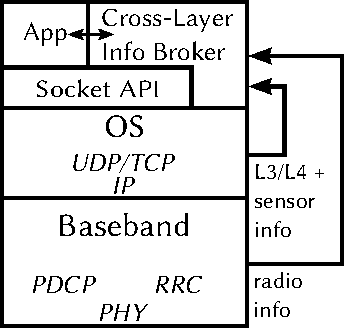
\includegraphics[width=0.25\textwidth]{images/cross-layer-model.pdf}
	\caption{Model and architecture of the proposed cross-layer information exchange.}
\label{c5:fig:crosslayer-model}
\end{figure}

Figure~\ref{c5:fig:crosslayer-model} illustrates the concept with the example of a mobile device. In a fully isolated model, no information would be passed from the baseband to the \gls{os} and the applications. The cross-layer model permits certain information to pass from one layer to another. Here, a software broker is responsible to collect information from several sources and layers and make it available to any interested application in a concise manner. 

This is an indirect cross-layer approach bypassing the intermediate layers completely and leaving them mostly unmodified. Also, information is always collected and used on the same device, making it purely vertical and distributed. Sharing this kind of information between different hosts would be accompanied by certain privacy and security implications. Most of the data is very sensitive and can also be used with malicious intent if it is being leaked by a cross-layer broker.

This architecture is intended to pass data from the physical and link layer directly up to the application. Especially information specific to \gls{3G} mobile networks could be potentially interesting and used in benefit for applications and the user experience.This could include:

\begin{itemize}
	\item Information on the occurrence of a horizontal handover between cells.

	\item Information on neighboring cells and predictions when a handover is most probable to occur.

	\item Information on the prediction of the occurrence of a vertical handover and thereby changes in the active network stack, e.g., to the WiFi layers.

	\item Information on the current signal strength, bit error rate, and throughput.

	\item Detailed mobility information, including current location and travel speed in relation to base station positioning and availability.
\end{itemize}

Today, most of this information is only available inside the link layer or even just known to the mobile network's control plane. The impact of a lack of this knowledge can be significant for applications. For example, traffic scheduled during a handover period can be subject to especially high latency and loss due to the lengthy control plane interactions and traffic rerouting processes in a mobile network. If a cross-layer exchange would be provided and the application is made aware when an handover is supposed to occur, traffic could be scheduled around the event. 

Generally speaking, the goal of the cross-layer approach would be to find meaningful reactions for every type of state the lower layers report through the broker. The pool of recipients is also not necessarily limited solely to the application layer. Especially the transport layer could be interested into explicit connectivity information and be modified to react accordingly. In addition to information flow, a path for control flow could also be envisioned. Herein, applications could directly influence the decision making and policies of the lower layers and adapt them to their personal needs.

All in all, the cross-layer data needs as well as the recipient's reactions need to be well defined and thoroughly tested to avoid any conflicts and layer separation issues. The impact of a simple unidirectional information flow on the layering mechanisms is suggested to be rather low. Only explicit and specific information is revealed keeping most of the isolation intact. However, a bidirectional control flow could soften up the isolation and have adverse side-effects through conflicting interests of participating applications.

Either way, when implementing any kind of cross-layer exchange, one always has to keep a close look on the resulting consequences. One side effect can be the creation of an unintentional feedback loop between the control mechanisms of protocols of different layers. Moreover, breaches in the isolation could leak network state that could be exploited by malicious parties in any number of unforeseeable ways. Therefore, handling these plays an important role in cross-layer research. In \cite{1404568} the authors present and discuss some of these issues.


%%%%%%%%%%%%%%%%%%%%%%%%%%%%%%%%%%%%%%%%%%%%%%%%%%%%%%%%%%%%%%%%%%%%%%%%%%%%%%%%
\subsection{Utilizing Cross-Layer Information for Adaptive Reliable Streaming in Mobile Networks}

Looking at the model it can be an obvious fit for adaptive reliable streaming. As introduced in Section~\ref{c3:sec:background}, adaptive streaming usually facilitates a segment-based pull approach on top of \gls{HTTP}. A local video buffer is maintained and attempted to be kept between predefined thresholds. The goal is to never run out of buffered video while still providing the best possible quality, which could be difficult to achieve in a highly variable mobile network.

Cross-layer information can be fed into the adaptivity model of the streaming player to better decide the exact schedule and quality level of segment transmissions. Adaptive reliable streaming can be especially suited to receive cross-layer data for several reasons: First, all requests are client-initiated, so available information can be immediately taken into account and does not need to be transfered elsewhere. Second, adaptive streaming consists of small and independent video segments, which allows to quickly react on upcoming events.

\begin{figure}[htb]
	\centering
	\begin{subfigure}[b]{0.80\textwidth}
		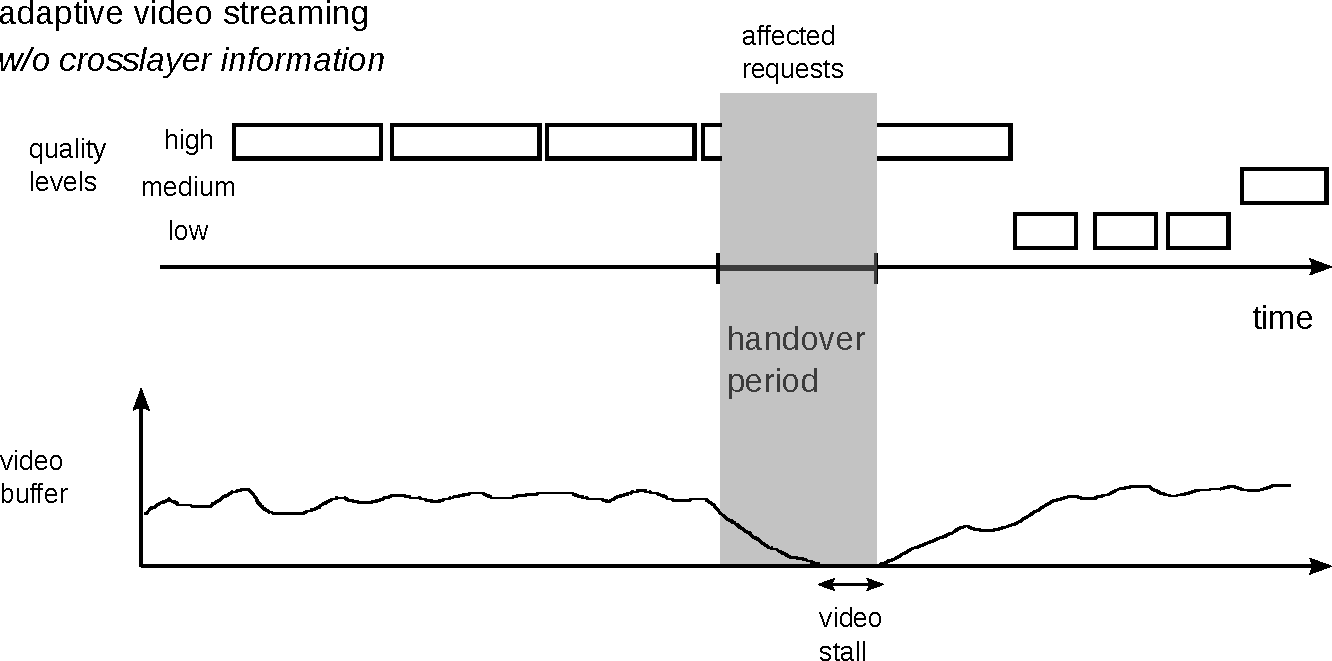
\includegraphics[width=\textwidth]{images/adaptive-streaming-no-cl.pdf}
		\caption{Stalling occurs without handover hinting.}
		\label{c5:fig:streaming-hinting-no-cl}
	\end{subfigure}%

	\begin{subfigure}[b]{0.80\textwidth}
		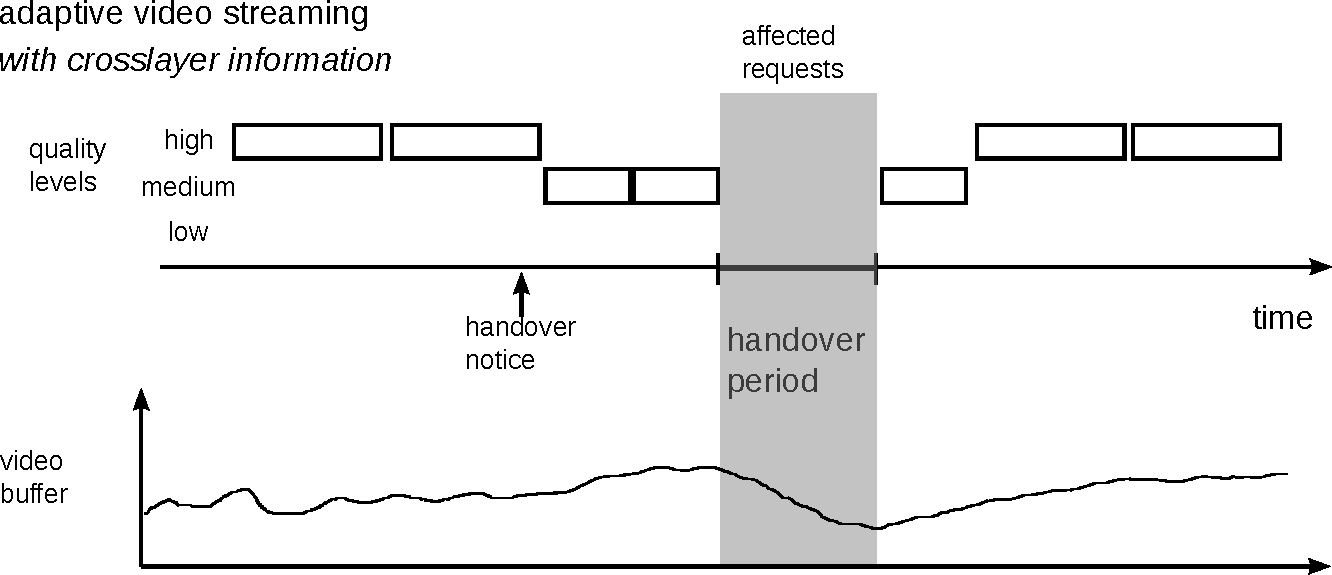
\includegraphics[width=\textwidth]{images/adaptive-streaming-cl.pdf}
		\caption{Stalling can be prevented by hinting and proactively filling the playback buffer.}
		\label{c5:fig:streaming-hinting-cl}
	\end{subfigure}%
	\caption{Adaptive video streaming scenario with and without handover prediction and cross-layer hinting.}
\label{c5:fig:streaming-hinting}
\end{figure}

One of the easiest events to improve upon is the timely knowledge (or prediction) of upcoming handover procedures, horizontal as well as vertical handovers. Consider the scenario given in Figure~\ref{c5:fig:streaming-hinting-no-cl}. The streaming player consistently retrieves video segments at the highest quality, maintaining a moderate buffer size but is oblivious to the upcoming handover. This handover interrupts any transmission for a certain time, during which the buffer is fully drained and the video playback begins to stall. Only after this phase ends, the remaining portion of the segment can be received. But the buffered amount is now still below the safety margin and the player is forced to request several segments in the lowest quality to quickly refill the buffer. Only after that, the player's state normalizes and normal quality playback is restored. In summary, one unexpected service interruption causes one complete stall and a long period of reduced quality in this exemplary scenario. This effect can also be easily observed in the mobile reliable streaming simulation scenario described in Section~\ref{c6:sec:mobilitystreamingsim}.

Figure~\ref{c5:fig:streaming-hinting-cl} shows the same scenario but with cross-layer hinting present. As soon as the notice of a predicted upcoming handover is received, the streaming player can react and switch to segments with medium quality to increase the buffer size before the event. After the handover has completed one more medium segment is transmitted to get the buffer level back to normal before returning to full quality. Both the video stalling period and the drop to the lowest quality could be avoided here. The general goal in the streaming process is to both stop the buffer from ever completely emptying and also maintaining the highest possible video quality. To achieve this, early knowledge of future network conditions is highly desirable for the streaming controller to correctly adjust the segment retrieval rate and quality.

The end-to-end concept can be applied to cross-layer architectures as well. While cross-layer information can still be made available to intermediate layers, the achievable effects might either not be as large as in the highest layer or more complicated to attain. For example, it requires much more effort to correctly adjust \gls{TCP} retransmissions and congestion control to accommodate the cross-layer broker without side-effects to other applications. Nonetheless, benefits can still be attained at the transport layer to some degree if the adjustments are being kept application-neutral. This can be especially helpful for applications that have not yet been adapted to handle cross-layer information.


%%%%%%%%%%%%%%%%%%%%%%%%%%%%%%%%%%%%%%%%%%%%%%%%%%%%%%%%%%%%%%%%%%%%%%%%%%%%%%%%
\subsection{Benefits for Other Applications}

Beyond this work's central motifs of reliable streaming, other applications could benefit as well. First, cross-layer information could be utilized to directly improve the user interface and experience. Any information of upcoming service interruptions or other adverse conditions are simply displayed to the user. This is specifically helpful for interactive communication --- as in video calls or \gls{VoIP}. An unsuspecting user might be more startled at a sudden loss of reception than the one that was informed beforehand. The communication partner can additionally also be informed. While user hinting and notifications does generally not actually improve the actual \gls{QoS} of the application it can still positively improve the perceived quality or \gls{QoE}. But detailed user studies would need to verify this further.

Generally, any application that can locally exert control over its traffic and does not have to rely on server-side control will benefit the most. Also, the traffic should ideally be composed of smaller objects available in multiple versions and free to be reordered. A good candidate would be Web browsers with their stateless \gls{HTTP} requests of a Web site, which is comprised of many small objects that can be, to a certain degree, requested in any order. Those objects could be requested in such an order to better accommodate network events announced by the lower layers. On the other hand, \gls{rtp}-style streaming traffic might not be able to beneficially utilize cross-layer information as just a stream of continuous data is pushed to onto the client.

Directly involving the user itself are a further category of cross-layer interactions that are only available if there is a downward control flow through the broker to the radio layer protocols. This would require the additional presence of a user-space policy manager. The manager would offer the user a series of preferences and a configuration interface for a rule-based cross-layer control engine. With this the user could create complex compound policies such as: ``Do not handover to a stationary WiFi from \gls{3G} when moving faster than \SI{50}{\kilo\meter\per\hour}, switch only to in-vehicle WiFi if available.'' or ``Avoid any vertical handover, which would interrupt my service for a long time, while a \acrshort{VoIP} call is running.''


%%%%%%%%%%%%%%%%%%%%%%%%%%%%%%%%%%%%%%%%%%%%%%%%%%%%%%%%%%%%%%%%%%%%%%%%%%%%%%%%
\subsection{Implementation Outlook and Approaches}

As the model displayed, the target applications should not be directly (or indirectly through the inclusion of a third-party software library) responsible to retrieve cross-layer information. Instead, the broker was suggested as the means to implement cross-layer exchange in an actual software environment. This daemon --- located in the user space --- collects information from the lower layer network protocols which usually reside entirely in kernel space. The kernel typically exposes only some data publicly with a stable \gls{API} and \gls{ABI}. Other data can often be derived from internal data structures which usually change with every version. The task of adapting to this changes and collecting concise data is handled by the daemon. Only the actual reactions to these information points must be implemented in the application itself.

The daemon provides all information through a pre-defined user space interface to interested parties. This includes the raw data itself, e.g., current latency or bandwidth information, as well as derived and predicted data points. Examples for the latter are the discussed early handover warning or mobility predictions. To further improve predicted values the daemon also integrates data from other device sensors outside the classical network stack, amongst others location and movement data and as well as system and battery state.

To further decouple the applications from the broker, the information should be provided through a shared \gls{IPC} bus. Current candidates for the reference implementation are Android, using the provided Intent\footnote{\url{https://developer.android.com/reference/android/content/Intent.html}} \gls{IPC} mechanism, as well as Linux distributions using D-Bus\footnote{\url{http://www.freedesktop.org/wiki/Software/dbus/}}. An even higher level implementation might be possible for the latter case, as the D-Bus-based NetworkManager\footnote{\url{https://wiki.gnome.org/Projects/NetworkManager}} framework already provides some of the network-related functionality. For example, it would be rather simple to implement switching the active network interface on the basis of cross-layer data with NetworkManager.

Through these decoupling efforts the broker's implementation and binary package can be completely swapped with another and all applications would still work as long as the bus interface stays the same. Therefore, the user and her chosen applications is not bound to a specific cross-layer broker provider with predictions conducted by certain algorithms. Rather, she can easily supplant the existing provider with a better one. The planned broker is therefore only meant as a reference implementation. Additionally multiple brokers could even be simultaneously active as long as as long as their provided data does not intersect.

The viability of cross-layer information can be evaluated in several ways. A pure network-level simulation can give initial hints on performance gains and issues. But only the evaluation of data traces and packet level captures of an actual reference implementation might give good insights into the implications of diminishing the network stack's layer encapsulation properties. A further comparative statistical analysis of several different approaches to cross-layer data predictions algorithms as well as the specific application's reactions could also prove to be of significant interest. Both the testbed and \gls{LTE} simulation approaches developed in Section~\ref{c6:sec:mobilestreamingtestbed} can help in validating this cross-layer approach.



% influence of signaling plane and core network elements - scaling
%This can apply to, e.g., reliability, frame sizing and fragmenting, and latency amounting to undesired effects on higher-layer traffic. 

 %Modem Link Properties Advertisement Protocol\footnote{\url{https://tools.ietf.org/html/draft-ivancic-mobopts-modemlpa-01}}

%LCP Link Control Protocol, PPP extension RFCs \cite{rfc1570,rfc1661}
%LISP and other mobility approaches \cite{rfc6830}

% Conceptually similar to cross-layer interactions is the family of dynamic radio resource management techniques. These control many properties concerning radio resources. 
% Radio Resource Management RRM
% 		\begin{itemize}
% 			\item resource monitoring, decision making, decision enforcement
% 			\item choose available wireless interfaces  best suited for a specific task
% 			\item rudimentary implementations in mobile OSs
% 		\end{itemize}
%	IEEE 802.21 cooperative handovers, but with required network support
%  Cross-layer design for wireless networks \cite{1235598} keine wirkliche aussage zu cross-layer

% User-centric mobility management for multimedia content access \cite{bolla2011usercentric} (not really cross-layer, uses something similar to LISP: an additional identifier shim and session migration for rtsp/sip) oddly mixed with user questionnaires

% Socketless \gls{TCP} --- an end to end handover solution \cite{1635680} % mobility scheme, not actually cross-layer information

%A ubiquitous mobile communication architecture for next-generation heterogeneous wireless systems \cite{1452832} (supposed to propose a function that determines the best handover initiation time in order to avoid early or late initiations)



	% - Research objectives
	% 	- Bidirectional vertical information and control flow on the performance of the individual layers
	% 		- Definition of generic interfaces
	% 		- Definition of a protocol (including information types, etc.)
	% 	- Definition of meaningful actions/reactions on the individual layers (e.g. adaptation of real-time communication data sources or changes in resource allocation)


%Using current location data and movement patterns/predictions to improve cell selections and initiate horizontal and vertical handovers to a time suitable for the device and running applications.


% For example, a Web browser could reorder its Website object requests to avoid sending any requests during handover periods and experience additional delay as seen in Figure~\ref{c5:fig:http-reorder}.
% 	\begin{figure}[htb]
% 	        \centering
% 	        \begin{subfigure}[b]{0.90\textwidth}
% 	            \centering
% 				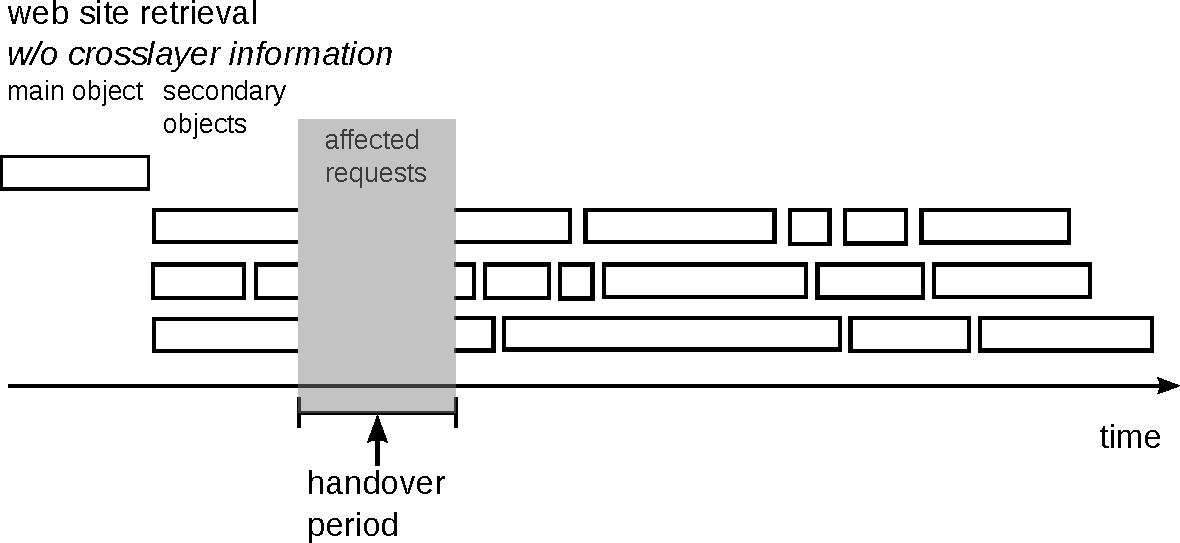
\includegraphics[width=\textwidth]{images/http-reorder-no-cl.pdf}
% 				\caption{The handover will block currently active object transmissions, page display will be delayed.}
% 				\label{c5:fig:http-reorder-no-cl}
% 	        \end{subfigure}%

% 	        \begin{subfigure}[b]{0.90\textwidth}
% 				\centering
% 				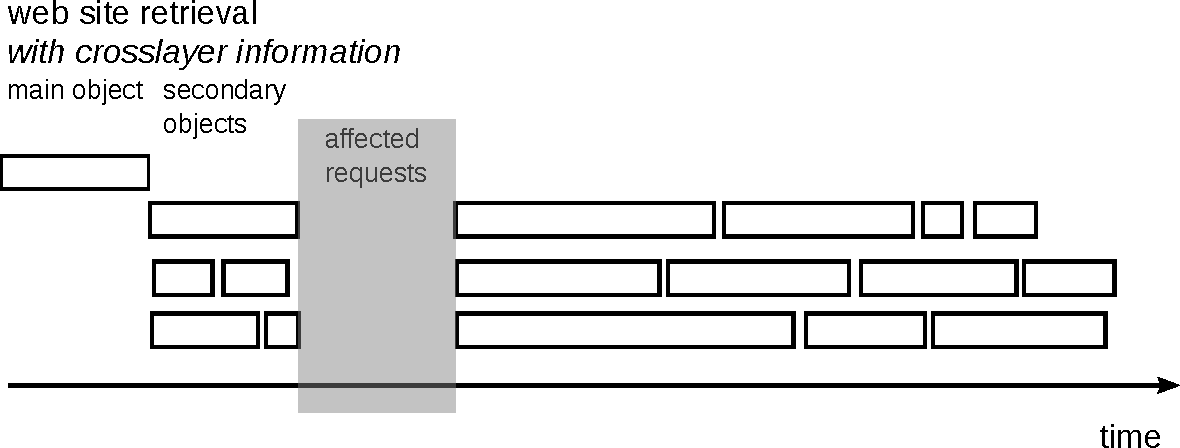
\includegraphics[width=\textwidth]{images/http-reorder-cl.pdf}
% 				\caption{The browser reorders the objects to be retrieved and avoids any transmissions during the indicated handover period.}
% 				\label{c5:fig:http-reorder-cl}
% 			   \end{subfigure}%
% 	 \caption{Mock-up of \gls{HTTP} reordering with handover awareness.}
% 	\label{c5:fig:http-reorder}
% 	\end{figure}



%Put into relation:
% \begin{itemize}
% 	\item frequency of handovers / distance/density of radio towers vs scenario traveling speed
% 	\item bit-length of streaming segments, typical transmission speed
% 	\item typical video length and number of segments
% 	\item derive number of interruptions in segments due to handovers
% 	\item estimate typical handover/mobility duration and service interruption time per event
% 	\item sum it up and compare to crosslayer information or even application layer handover decision
% \end{itemize}